% ===== 原文 pp.1–3（PDF p.11–13） =====

\chapter{引言与概述}

\section{电磁对偶、几何朗兰兹与 Kapustin--Witten 的工作}

% [原文 p.1]

Maxwell 写下电磁学方程后不久，人们就注意到：把电场与磁场互换，方程的形式保持不变——
只要同时把带电荷的源与带磁荷的源互换。用数学语言说，这个对偶操作不过是把电磁场强
2-形式 $F$ 与其 Hodge 对偶 $\star F$ 互换。

然而，二十世纪物理学的发展方向在形式上遮蔽了 Maxwell 方程的这一底层对称性。
把电磁学改写为规范理论（即，把电磁场等同于时空上一个主 $U(1)$ 丛上的联络 $A$）之后，
对偶性就不再显然，因为 2-形式 $F=\dd A$ 与其 Hodge 对偶 $\star\dd A$ 在这一形式体系中
扮演着极不相似的角色。特别地，电性源与磁性源的引入方式非常不同：电性源成为
\emph{Wilson 线}有序算子，作为作用量中的源项出现；而磁性源成为 \emph{'t Hooft 线}
无序算子，通过在场构型空间中强加一个预先给定的奇异性来引入。电磁对偶最终可以推广到
$U(1)$ 联络的量子理论；这一等价性虽然仍可证明 [8]，却被形式体系遮蔽得更深了。

% [Tutor Note: p.1 “电磁场强 2-形式”与“联络”的区别需注意：$F=\dd A$ 是整体定义的闭 2-形式，
%  而 $A$ 只在局部（或在一个主丛的平凡化下）有定义；$U(1)$ 情形下 $[\dd A]\in H^2(M;\Z)$
%  才是规范不变的（第一陈类）。这是 Maxwell 理论作为“$U(1)$ 联络的规范理论”与“2-形式场论”的差别所在。]

对于非阿贝尔规范群 $G$，电磁对偶的一个版本可以推广到某个特定的四维量子规范理论，
即 $\cN=4$ 超对称杨--米尔斯理论（我们在第 2 章回顾）。在这一情形中，这一等价性
（称为 \emph{S-对偶}）远为不平凡——不平凡到了获得数学力量的程度。也就是说，
用来描述对偶结构的语言采取了如此不同的形式，以至于它们的等价性从纯数学的观点看
也极有意义。本论文即致力于研究 S-对偶的某些数学推论。

在写下这类数学预言时，人们首先会遇到非阿贝尔对偶的一个显著特征：规范群为 $G$ 的
$\cN=4$ 理论被映到规范群为 $\LG$（称为朗兰兹对偶群）的 $\cN=4$ 理论；

% [原文 p.2]

$G$ 与 $\LG$ 通过交换它们的特征标格与余特征标格相联系，一般说来是不同的李群。
因此，比较对偶的两边，就是比较由朗兰兹对偶李群对所标记的数学结构。

恰巧，李群对 $G$ 与 $\LG$ 也出现在数论的一组深刻猜想与定理之中，这些猜想与定理合起来
被称为\emph{朗兰兹对应}。这些猜想可以有多种推广与表述方式，但其核心在于：朗兰兹对应的
每一版本都假设，由一个李群 $\LG$ 标记的某个数学对象（我们可称之为对偶的“A-侧”）
与另一个涉及对偶群 $G$ 的对象（可称之为“B-侧”）之间存在同构。
（关于朗兰兹纲领的更多内容，见 [7] 及其中的参考文献。）

% [Tutor Note: p.2 这里的 A/B 标记法与通常的几何朗兰兹文献（如 Frenkel 的综述）一致：
%  A-侧由 $\LG$ 标号（在 $\Bun_{\LG}C$ 上的 $\cD$-模），B-侧由 $G$ 标号（$C$ 上与 $G_\C$ 联络相关的对象）。
%  注意后文 §1.1 把 $t=1$ 扭转（规范群 $\LG$）称 A-侧、$t=\ii$ 扭转（规范群 $G$）称 B-侧，与此处一致。]

例如，朗兰兹对应的一个形态（与物理最直接相关的那个）被称为\emph{几何朗兰兹}，
它断言与给定（闭、定向）黎曼面 $C$ 相联系的两族对象是等价的：
\begin{equation}
  \eqbox{Hecke 特征层\\（$\cD$-模的）在 $\Bun_{\LG}C$ 上}
  \;\longleftrightarrow\;
  \eqbox{$C$ 上的平坦（不可约）\\ $G_{\C}$-丛} \tag{1.1}
\end{equation}

B-侧是 $C$ 上配以平坦联络的主 $G_{\C}$-丛的集合，其中 $G_{\C}$ 是李群的复化；
等价地说，它是同态 $\pi_1(C)\to G_{\C}$ 的集合。一般地，这个集合构成一个有限维
模空间 $\cM_{flat}(G_{\C},C)$。A-侧稍微更抽象一些：$\Bun_{\LG}C$ 是 $C$ 上全纯
$\LG$-丛的空间，\footnote{实际上，由于 $\Bun_{\LG}C$ 的奇异性，严格说来它是一个
“模堆”（moduli stack）而不是一个“空间”。}在其上定义了微分算子层的模，即
\emph{$\cD$-模}。猜想是：对 $C$ 上的每个平坦 $G_{\C}$-丛，都有相应的 $\cD$-模层——
不仅是某个层，而是某个“Hecke 变换”的“特征层”。

% [Tutor Note: p.2 式 (1.1) 中 $\cD$-模与“Hecke 特征层”的含义（供核对）：
%  Hecke 对应是 $\Bun_{\LG}C$ 上的一族对应（对每一点 $x\in C$ 与每个表示 $V$，把一个 $\LG$-丛
%  “在 $x$ 处作修正”），它作用在 $\cD$-模的（导出）范畴上；所谓“特征层”，是指在该作用下
%  本征值为某个特征标（与一个 $G_\C$-局部系对应）的 $\cD$-模。几何朗兰兹的精确陈述是这两族对象之间
%  （带相容性）的等价，而非简单的双射。]

先不论上一句中引号里的那些词的确切定义，让我们指出关于几何朗兰兹的上述数学陈述的
几个特征，它们恰好会推广为贯穿本论文的宽泛主题：
\begin{itemize}[leftmargin=1.6em,itemsep=2pt,topsep=2pt]
\item 在上面的右边方框中，我们遇到的是黎曼面 $C$ 上的平坦、复化联络。确实，这类联络在
  本论文各处的好几个语境中自然地出现；它们的出现是几何朗兰兹对应 B-侧的标志。
\item 上面的左边方框中的结构，要精确描述它们需要多得多的词与概念，远多于右边方框中相应
  的结构。的确，一般说来，几何朗兰兹对应的 A-侧比 B-侧远为难以给出严格而简单的数学定义。

% [原文 p.3]

\item 某些奇特的数学定义（例如上述“特征层”与“Hecke 变换”的概念）具有生动的物理实现 [1]，
  这提示物理也许能为表述这一对应提供最自然的语言。
\end{itemize}

成对出现的对偶李群使 M. Atiyah 早在 1977 年就猜测 [1]：规范理论的 S-对偶可能与
几何朗兰兹有关。这一猜想最终在 A. Kapustin 与 E. Witten 的开创性论文 [1] 中实现：
他们证明，几何朗兰兹对应来自 S-对偶应用于一个非常特殊的物理设置。具体地说，
他们考虑由 $\cN=4$ 经一种涉及复扭转参数 $t$ 的扭转程序构造出的某个拓扑场论（TFT）。
（我们在下一章描述这一扭转程序与 $t$ 参数。）他们关注 $t$ 的两个特殊值，分别对应
朗兰兹对应的两侧：A-侧是 $t=1$、规范群为 $\LG$ 的扭转理论，而 B-侧是
$t=\ii$、规范群为 $G$ 的扭转理论。\footnote{对于零 $\theta$ 角与倒转的耦合强度。}
时空选为两个黎曼面的乘积
\begin{equation*}
  M=\Sigma\times C
\end{equation*}
（其中闭黎曼面 $C$ 的亏格 $g_C$ 取为满足 $g_C\ge 2$），他们考虑 $C$ 的尺寸收缩到零的极限。

% [Tutor Note: p.3 此处 [1] 即 Kapustin–Witten 的论文；Atiyah 1977 年的猜想通常被引作
%  Atiyah 关于 S-对偶与几何朗兰兹之间联系的早期洞见（见 KW 论文引言中的转述）。若需原始出处，
%  应另行核对 Atiyah 1977 年的工作，不能把 [1] 当作 1977 年的文献。]

\begin{figure}[htbp]
\centering
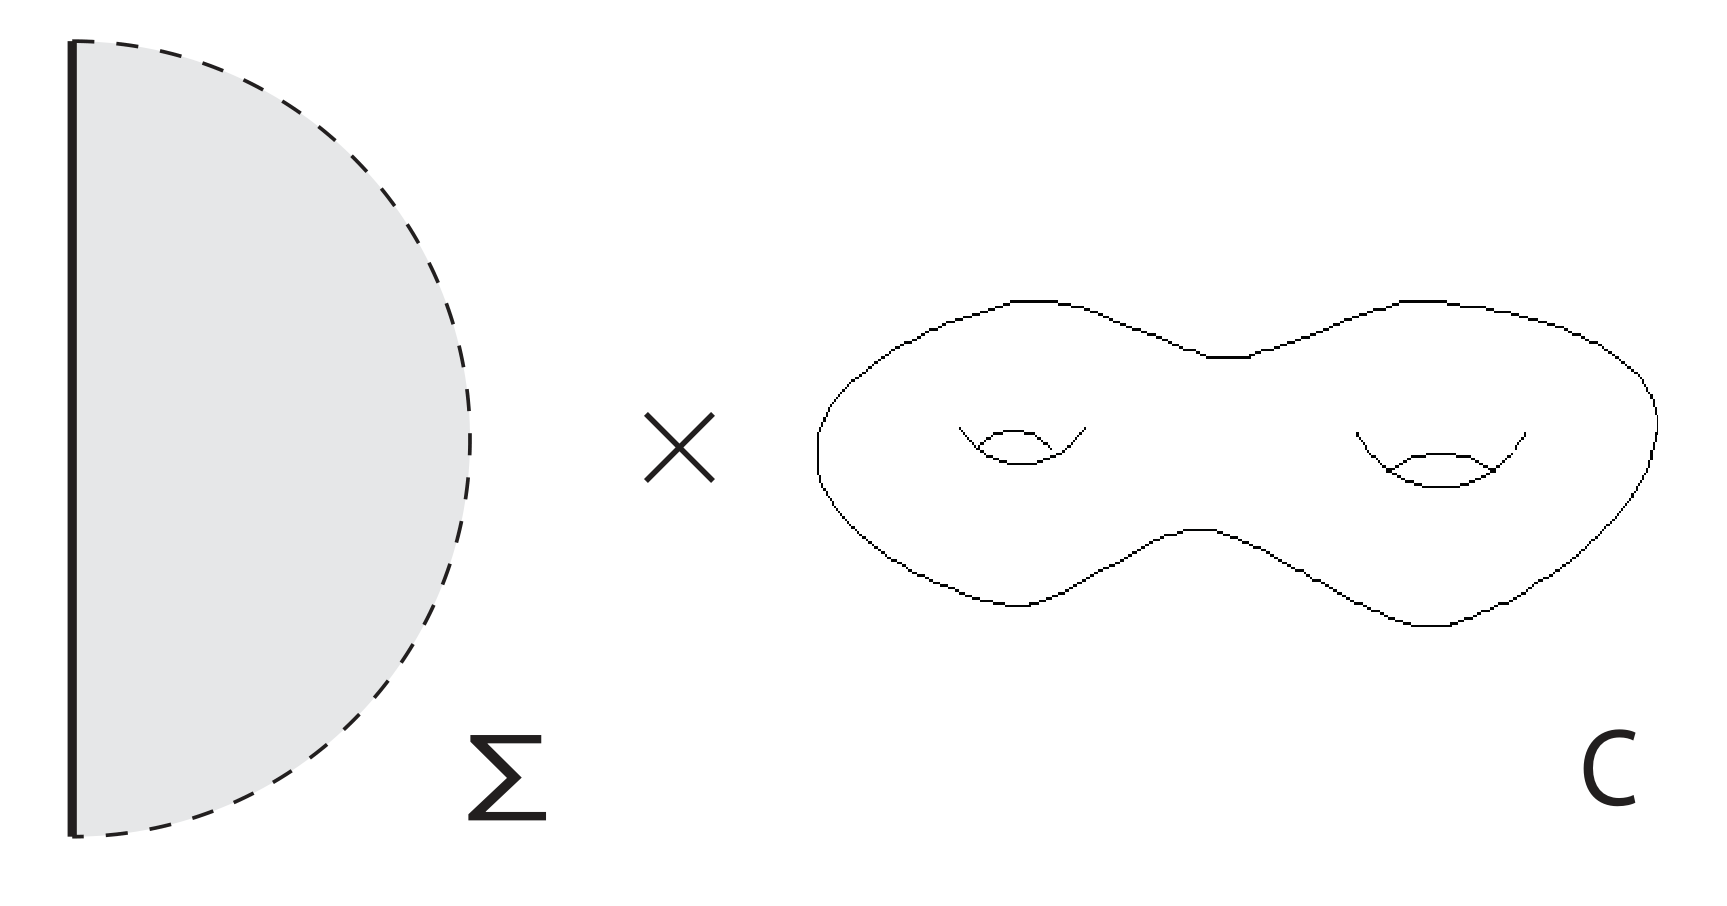
\includegraphics[width=0.62\textwidth]{fig11.png}
\figtitle{1.1}{扭转理论被放在乘积流形 $\Sigma\times C$ 上，而 $C$ 的尺寸被收缩到零。}
\end{figure}

在这一极限下，扭转理论约化为 $\Sigma$ 上的有效 2d TFT：在 A-侧，$t=1$ 的理论约化为
$\Sigma$ 上的拓扑 A-模型（在 §7.1 回顾），这个理论唯一的玻色场是从 $\Sigma$ 到某个
辛靶空间的映射。此情形下的靶空间是 Hitchin 模空间 $\cM_H(\LG,C)$，它是一个超 Kähler流形，维数为
\[
  \dim\cM_H(\LG,C)=4(g_C-1)\dim\LG
\]

% [Tutor Note: p.3 维数公式核对：Hitchin 模空间在复结构 $I$ 下同构于 $T^*\cM_{flat}$，
%  而 $\dim_\C\cM_{flat}(G,C)=(g-1)\dim G$（对紧群 $G$），故 $\dim_\C\cM_H=2(g-1)\dim G$，
%  实维数为 $4(g-1)\dim G$，与原文一致。注意 $\LG$ 与 $G$ 有相同的李代数维数。]
